%!TEX root =  ../main.tex

\subsection{Restrained Growth}

\objective{Create and use logistic curves}


Exponential growth can rarely be carried on for long.  Bacteria fill the petri dish, 
bunnies eat all the grass, and the shower-water has a maximum heat it can 
reach.  In every case, the is a constraint, a ceiling value that the population 
cannot grow beyond.  Typically, it is approached asymptotically.  This means there are
two horizontal asymptotes.  The left half of the graph is concave up (exponential
growth) and the right half is concave down (logarithmic growth).  

How can these graphical quantities be achieved algebraically?  What can 
be done to $y=e^x$ to make it have a horizontal asymptote?  As we saw last
chapter, rational functions have horizontal asymptotes at the level of the ratio
of the numerator to the denominator ``at infinity''.  So we need to create a 
denominator.  But we don't want the denominator to ever equal 0, lest we
create a vertical asymptote.  Dividing by $e^x$ is almost right.  Let's make it
$e^x+1$.

$$
f(x) = \frac{e^x}{e^x+1}
$$

\begin{figure}[h]
\begin{centering}
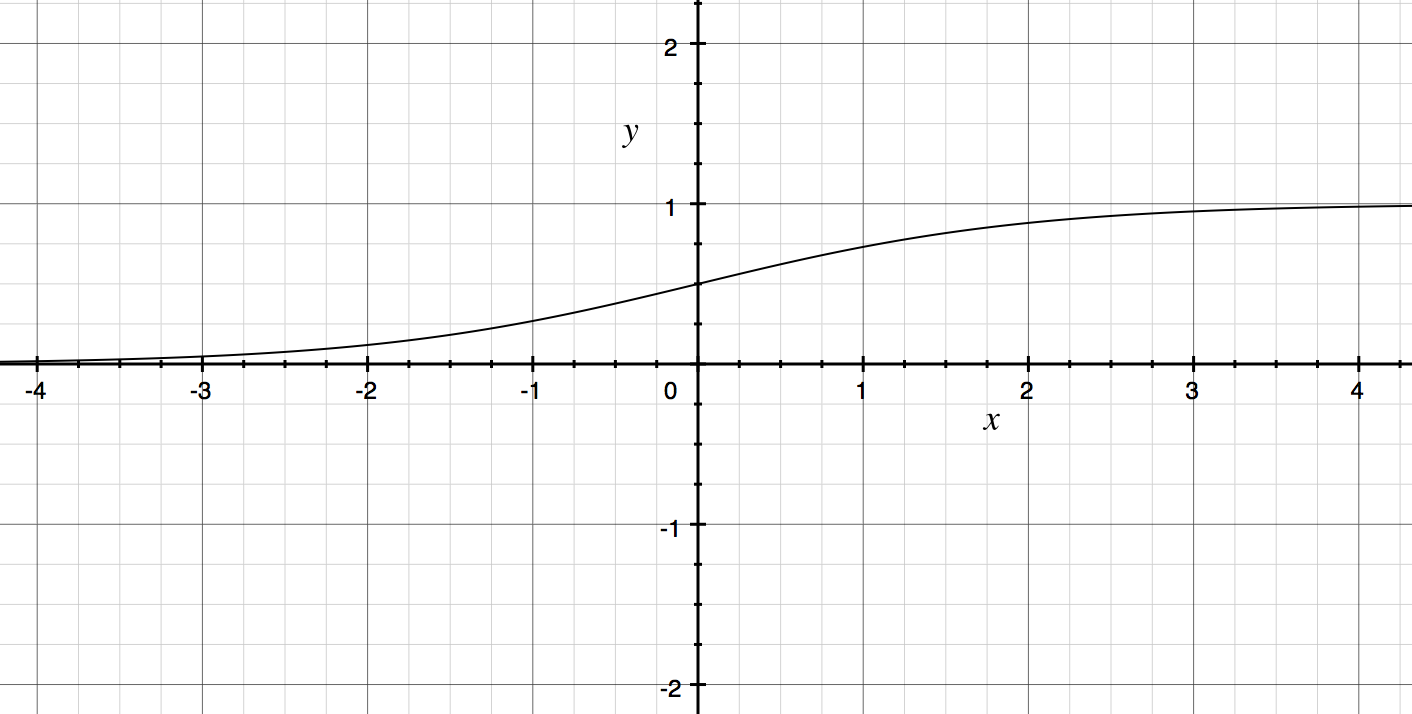
\includegraphics[scale=0.5]{\chapdir/pics/basicalogistic}
\caption{A basic logistic curve}
\end{centering}
\end{figure}

That worked out nicely, but it made our equation slightly more complicated
than we might otherwise like.  If we want to do any inside transformation (e.g.
shift left/right, widen/narrow) then we will need to modify $x$ in two places.  Can
we consolidate the $x$ to be in only one place?  What could we do to the
numerator and denominator ?

Dividing top and bottom by $e^x$ will cancel the two terms with $x$ in them.
Furthermore, we can eliminate the need for complex fraction by changing
a denominator under 1 to be a negative exponent.

$$
f(x) = \frac{1}{1+e^{-x}}
$$

Notice which numbers control the behavior of the graph.  The 1 in the numerator
is the maximum height of the graph, which typically called $c$ for ceiling. If we
insert a multiplying constant next to $x$ in the exponent, it will contract the
graph in the $x$-direction, making the curve of the S steeper.  If we insert
a multiplying constant next to x, it will shift the turning point to the right.  No
matter what we do, the inflection point will occur half-way up.

$$
f(x) = \frac{c}{1+ae^{-bx}}
$$

\subsection{Regression}
The TI-8* has a LOGISTICREG function which is excellent for computing
regressions of this kind, and outputs functions of the kind already discussed.
However, if we need to make an equation ourselves by hand, $e$ is slightly
awkward number to use.  Algebra manipulation is much easier with this
equation:

$$
f(x) = \frac{c}{1+ab^{-x}}
$$
